% This work is licensed under the Creative Commons
% Attribution-NonCommercial-ShareAlike 4.0 International License. To view a copy
% of this license, visit http://creativecommons.org/licenses/by-nc-sa/4.0/ or
% send a letter to Creative Commons, PO Box 1866, Mountain View, CA 94042, USA.

\newcommand{\directoryPrefix}{../latex/} % Je nach Ordnertiefe muss dieser Command angepasst werden. Bei Fragen mich anschreiben.
\input{\directoryPrefix templates}
\TemplateSummary{Willi Sontopski}{WTHM}

\begin{document}
	\section{Bedingter Erwartungswert (nicht direkt prüfungsrevelant)}
	\begin{itemize}
		\item Bedingter Erwartungswert als $L_2$-Projektion auf abgeschlossenen Unterraum $L_2(\Omega,\F,\P)\ni\E[X|\F]$, $\gdw\langle X-\E[X| \F],F\rangle=0~\forall F\in L_2(\F)$; hat eindeutige stetige Fortsetzung auf $L_1$
		\item $X\in\L_2(\F)\implies\E[X|\F]=X$ "$X$ ist $\F$-messbar"
		\item $\E[a\cdot X+b\cdot Y|\F]=a\cdot\E[X|\F]+b\cdot\E[Y|\F]\qquad\forall a,b\in\R$ (Linearität)
		\item $\langle\E[X|\F],Y\rangle=\langle X,\E[Y|\F]\rangle=\langle\E[X|\F],\E[Y|\F]\rangle$ (Symmetrie, gilt nur in $L_2$)
		\item $\E\big[\E[X|\F]\big|\mathcal{H}\big]=\E[X|\mathcal{H}]$ für $\mathcal{H}\subseteq\F\subseteq\A$ (Turmregel)
		\item $\E[Z\cdot X|\F]=Z\cdot\E[X|\F]$ für alle $Z$ beschränkt und messbar (also z.B. $Z\in L_2$) (Pull-Out-Property)
		\item $X\leq Y\implies \E[X|F]\leq\E[Y|\F]$ (Monotonie)
		\item $\big|\E[X|\F]\big|\leq\E\big[|X|\big|\F\big]$ (Dreiecksungleichung)
		\item $Y=\E[X|\F]$ f.s. $\Longleftrightarrow\forall F\in\F:\E[X\cdot\indi_F]=\E[Y\cdot\indi_F]$
		\item $\E[X]=\E\big[X\big|\lbrace\emptyset,\Omega\rbrace\big]$ und außerdem $\E\big[\E[X|\F]\big]=\E[X]~\forall\F\subseteq\A$ (totaler Erwartungswert)
		\item $B_b(\R):=\lbrace f:\R\to\R\mid f$ beschränkt und Borel-messbar$\rbrace$
		\item ZG $X$ \define{unabhängig von} $\F\subseteq\A$, i.Z. $X\unab\F:\gdw\E\big[f(X)\cdot\indi_A\big]=\E\big[f(X)\big]\cdot\P(A)~\forall A\in\F,\forall f\in B_b(\R)$
		\item ZG $X$ heißt \define{unabhängig von ZG} $Y$, i.Z. $X\unab Y:\gdw X\unab\sigma(Y)\gdw\E\big[f(X)\cdot g(Y)\big]=\E\big[f(X)\big]\cdot\E\big[g(Y)\big]~\forall f,g\in B_b(\R)$
		\item $X\unab\F\implies\E[X|\F]=\E[X]$; der andere Extremfall war $X$ $\F$-messbar $\implies\E[X|\F]=X$.
		\item $\E[X|Y_1,\ldots,Y_n]:=\E\big[X\big|\sigma(Y_1,\ldots,Y_n)\big]$ "Beste Vorhersage von $X$ gegeben $Y$."
	\end{itemize}
	
	\section{Martingale}
	\begin{itemize}
		\item ist "faires Spiel" zwischen zwei Personen, bei dem keine Strategie einen systematischen Vorteil bringt
		\item Familie $(\F_t)_{t\in I}$ von $\sigma$-Algebren $\F_t\subseteq\A$ heißt \textbf{Filtration} 
		$:\gdw( s\leq t\implies\F_s\subseteq\F_t)$; 
		ist aufsteigenden Folge von $\sigma$-Algebren.
		Interpretation: $\F_t$ beschreibt die zum Zeitpunkt $t$ verfügbare Information;
		Informationsfluss wächst mit der Zeit;
		$\F_\infty:=\bigcup_{t\in I}\F_t$.
		\item Ein \textbf{stochastischer Prozess (SP)} ist eine Familie $(X_t)_{t\in I}$ von Zufallsvariablen.\\
		Ein SP $(X_t)_{t\in I}$ heißt \textbf{adaptiert} an die Filtration $(\F_t)_{t\in I}$
		$:\gdw\forall t\in I: X_t$ ist messbar bzgl. $\F_t$
		\item Eine Folge $(e_n)_{n\in\N}$ heißt \textbf{vorhersehbar} bzgl. einer Filtration $(F_t)_{n\in\N}$
		$:\gdw\forall n\in\N:e_{n+1}$ ist messbar bzgl. $\F_n$
		Vorhersehbarkeit ist stärker als Adaptiertheit.
		\item Sei $X=(X_t)_{t\in I}$ SP und $(\F_t)_{t\in I}$ eine Filtration.
		$X$ heißt \textbf{Martingal} $:\gdw$
		\begin{enumerate}[label=(\alph*)]
			\item $(X_t)_{t\in I}$ ist adaptiert an $(\F_t)_{t\in I}$
			\item $\begin{aligned}
				X_t\in L_1(\Omega,\A,\P) \qquad \forall t\in I\qquad(\text{ d. h. } \E\big[|X_t|\big]<\infty)
			\end{aligned}$
			\item $\begin{aligned}
				\E[X_t~|~\F_s]=X_s\qquad\forall s,t\in I\mit s\leq t
			\end{aligned}\qquad$
			(Diskret:
		$ \E[X_{n+1}~|~\F_n]=X_n~\forall n\in\N$) 
		\end{enumerate}
		\item \textbf{Submartingal}: statt (c) gilt $\E[X_t~|~\F_s]\geq X_s$ (Der zukünftige Wert wird unterschätzt $\leadsto$ Gewinn)
		\item \textbf{Supermartingal}: statt (c) gilt $\E[X_t~|~\F_s]\leq X_s$ (Der zukünftige Wert wird überschätzt $\leadsto$ Verlust)
		\item \textit{"Das Leben ist wie ein Supermartingal - die Erwartung fällt mit der Zeit."}
		\item Die Sub-/Super-Eigenschaft hängt von Filtration ab.
		Ist $(M_t)_{t\in T}$ MG bzgl. $(\F_t)_{t\in T}$, dann auch bzgl. $(\F_t^E)_{t\in T}$ mit $\F_t^E:=(\sigma(M_s:s\leq t)$ (\define{erzeugte Filtration}
		\item Das von ZG $X$ und Filtration $(\F_t)_{t\in T}$ erzeugte MG ist $X_t:=\E[X|\F_t]$.
		\item Ein \define{Random Walk (RW) mit Schrittverteilung $F$} ist $S_N:=\sum_{i=1}^N\xi_i$ mit $(\xi_n)_{n\in\N}$ iid $\xi_1\sim F$.
		Heißt \define{symmetrisch}, falls $F$ symmetrisch; \define{einfach} falls $\P[\xi\in\lbrace-1,1\rbrace)=1$
		\item Ein RW ist Martingal, falls $\E[\xi_1]=0$; Sub-M., falls $\E[\xi_1]\geq0$; Super-M., falls $\E[\xi_1]\leq0$
		\item $X\wedge Y:=\min\lbrace X,Y\rbrace$ und $X\vee Y:=\max\lbrace X,Y\rbrace$
		\item Linearkombination von MG wieder MG; nichtnegative Linearkombination von Super/Sub-MG wieder Super/Sub-MG
		\item $M_n$ SubM $\gdw -M_n$ SuperM.; $X_t,Y_t$ SuperM $\implies X_t\wedge Y_t$ SuperM; $X_t,Y_t$ Sub-M $\implies X_t\vee Y_t$ SubM
		\item $X$ MG, $\phi$ konvex, $\E\big[\phi(X)\big]<\infty\implies \phi(X_t)$ ist SubM
		\item $X_t$ MG $\gdw X_t$ Super- und Sub-Martingal
		\item \define{Bedingte Jensen-U:} $\phi\big(\E[X|\F]\big)\leq\E\big[\phi(X)|\F\big]$ mit $\phi:\R\to\R$ konvex, $\E[\phi(X)]<\infty,~\F\subseteq\A$.
		\item \define{Doob-Zerlegung:} Jeder adaptierte SP $(X_n)_{n\in\N}$ lässt sich zerlegen in $X_n=X_0+M_n+A_n$ mit MG $M_n$ (mit $M_0=0$) und $A_n$ vorhersehbar $(A_0=0)$. Die Zerlegung ist fast sicher eindeutig.
		$X_n$ SubM $\implies A_n$ f.s. wachsend; $X_n$ SuperM $\implies A_n$ f.s. fallend.\\
		\textit{Beweis.} VÜ: DZ $\implies A_n=\sum_{j=1}^n\E\big[X_j-X_{j-1}|\F_j\big]$; Existenz: $M_n:=X_n-X_0-A_n$ ist MG; Eindeutigkeit: Laut VÜ Wahl von $A$ notwendig, also $A_n=A_n'\leadsto M_n=M_n'~\square$
		\item \textbf{Kompensator-Lemma:} Sei $(M_n)_{n\in\N}$ bzgl. $(\F_n)_{n\in\N}$ mit $\E[M_n^2]<\infty\implies M_n^2$ SubM \& $\exists!$ steigender vorhersehbarer SP (\define{Kompensator}) $\langle M\rangle_n$ so, dass $\big(M_n^2-\langle M\rangle_n\big)_n$ MG ist. Außerdem:\\
		$\E\left[(M_n-M_{n-1})^2~\big|~\F_{n-1}\right]=\langle M\rangle_n-\langle M\rangle_{n-1}~\forall n\in\N$\\
		\textit{Beweis.} $M_n^2$ ist SubMG wegen $\phi:x\mapsto x^2$ konvex; Doob-Zerlegung von $M_n^2$ ist\\
		$M_n^2=M_0^2+\underbrace{\big(M_n^2-\langle M\rangle_n-M_0^2\big)}_{=\tilde{M}_n\text{, Martingal}}+\underbrace{\langle M\rangle_n}_{\text{vorhersehbar + steigend}}$; Gl nachrechnen $\square$
		\item \define{Martingaltransformation} ist SP $(\vartheta\bullet M)_n:=\sum\limits_{i=1}^n\vartheta_i\cdot(M_i-M_{i-1}),(\vartheta\bullet M)_0:=0$
		mit $M_n$ (Sub-/Super-)MG und $\vartheta_n$ vorhersehbarer SP. Interpretation: $(M_n-M_{n-1})$ ist Gewinn in der $n$-ten Runde, $\vartheta_n$ ist Einsatz in $n$-ter Runde, MG-Trafo ist Gesamtgewinn nach der $n$-ten Runde mit Einsatzverhalten $\vartheta_n$.
		\item SP $\vartheta$ \define{lokal beschränkt} $:\gdw\exists(K_n)_{n\in\N}\subseteq\R:\forall n\in\N:\forall k\leq n:|\vartheta_k|\leq K_n$; beschränkt $\Rightarrow$ lokal bs.
		\item MG-Trafo: $M\mapsto(\vartheta\bullet M)$ und $\vartheta\mapsto(\vartheta\bullet M)$ sind linear; $M$ MG \& $\vartheta_n$ lokal beschränkt $\implies(\vartheta\bullet M)$ MG; $M_n,\vartheta_n\subseteq L_2\implies(\vartheta\bullet M)$ MG; faires Spiel bringt für beliebige Strategie $\vartheta_n$  keinen Vorteil (da wieder MG)
	\end{itemize}
	
	\section{Stoppzeiten und Stoppen von stochastischen Prozessen}
	\begin{itemize}
		\item \define{Stoppzeit (SZ)} $\tau:\Omega\to I\mit\lbrace \tau\leq t\rbrace\in\F_t~\forall t\in I\mit (\F_t)_{t\in I}$ Filtration.
		Interpretation: Zu jedem Zeitpunkt $t\in I$ wissen wir, ob $\tau$ bereits eingetreten ist $\lbrace\tau\leq t\rbrace$ oder nicht.
		\item Typisches Beispiel: Ersteintrittszeit von adaptierten SP $\tau(\omega)=\min\lbrace n\in\N_0:X_n(\omega)\geq k\rbrace$
		\item $\lbrace \tau=n\rbrace\in\F_n~\forall n;\lbrace \tau\geq n\rbrace\in\F_{n-1}~\forall n;\sigma\wedge\tau,\sigma\vee\tau$ sind SZ, $\inf_n\tau,\sup_n\tau_n$ sind SZ
		\item $X_\tau\colon\Omega\to\R,\qquad \omega\mapsto X_{\tau(\omega)}(\omega)\qquad\forall \omega\in\lbrace\tau<\infty\rbrace$
	und den \textbf{bei $\tau$ gestoppten stochastischen Prozess}
	$X_t^\tau(\omega):=:X_{t\wedge\tau}(\omega):=\left\lbrace\begin{array}{cl}
			X_t(\omega), & \falls \omega\in\lbrace t\leq\tau\rbrace\\
			X_{\tau(\omega)}(\omega), &\falls\omega\in\lbrace t>\tau\rbrace
		\end{array}\right.$
		Interpretation: $X_t^\tau=X_t$, falls die Stoppzeit noch nicht eingetreten ist und $X_t^\tau=$ konstant dem Wert zum Stoppzeitpunkt.
		\item Sei $(X_n)_{n\in\N}$ MG. Dann: $X_{n\wedge\tau}$ ist MG mit $\E[X_{n\wedge\tau}]=\E[X_0]$. \textit{Beweis.} Stoppen $\hat{=}$ MG-Trafo mit (lokal beschränktem) $\vartheta_{n}:=\indi_{n\leq\tau}\leadsto X_0+(\vartheta\bullet X)_n\leadsto\square$.
		\item "Es gibt keine Stoppzeit, sodass der gestoppte Prozess in einer anderen Klasse liegt als der Prozess" % siehe Wikipedia
		\item \define{Doobs Optional Stopping Thm:} Sei $(X_n)_{n\in\N}$ MG und $\tau:\Omega\to\N\cup\lbrace\infty\rbrace$ mit $\P[\tau<\infty]=1$. 
		Dann gilt $\E[X_\tau]=\E[X_0]$ in einem der Fälle: ("Stoppstrategie ändert nichts an Fairness")
		\begin{enumerate}
			\item $\tau$ f.s. beschränkt, d.h. $\exists K\in N_0:\P[\tau\leq K]=1$
			\item $X^\tau$ f.s. beschränkt, d.h. $\exists K>0:\P(\sup_{n\in\N_0}|X_{\tau\wedge n}|\leq K)=1$
			\item $\E[\tau]<\infty$ und "beschränkte Zuwächse": $\exists K>0:\P(\sup_{n\in\N_0}|X_{\tau\wedge n}-X_{\tau\wedge(n-1)}|\leq K)=1$
		\end{enumerate}
		\item \textit{Beweis.} a) folgt aus Satz zuvor; b) dominierte Konvergenz; c) Teleskopsumme + domKonv
		\item Stoppzeit \define{assoziierte $\sigma$-Algebra} ist $\F_\tau:=\lbrace	A\in\A\mid\forall t\in I:A\cap\lbrace\tau\leq t\rbrace\in\F_t\rbrace$ für SZ $\tau$ bzgl. $(\F_t)_{t\in I}$.
		\item $\F_\tau$ deterministisches Objekt; $\sigma\leq\tau\implies\F_\sigma\subseteq\F_\tau;~\lbrace\sigma<\tau\rbrace\in\F_\sigma\cap\F_\tau;~\F_\sigma\cap\F_\tau=\F_{\sigma\wedge\tau}$
		\item \define{Doob's optional sampling:} $(X_n)_{n\in\N}\subseteq L_1$ SP: TFSAE; a) $X_n$ ist MG; b) $\E[X_\sigma]=\E[X_\tau]~\forall\sigma,\tau$ beschränkt; c) $X_\sigma=\E[X_\tau|\F_\sigma]~\forall \sigma\leq\tau$ beschränkt (Satz gilt ähnlich für Sub-/Super-MG)
		\textit{Beweis.} a) $\Rightarrow$ b) folgt aus Doobs optional stopping a); c) $\Rightarrow$ a): konstant wählen
	\end{itemize}
	
	\section{Martingalkonvergenz und gleichgradige Integrierbarkeit (ggi)}
	\begin{itemize}
		\item VÜ: Für Folge $(a_n)_n$ gilt $\limn a_n$ existiert \betone{nicht} in $\overline{\R}\gdw(a_n)_n$ überquert unendlich oft aufsteigend den Streifen $[p,q]\times\N\gdw\exists p<q\in\Q:U[p,q]=\infty$
		\item $U_N[p,q]$ ist Anzahl Upcrossings auf $[p,q]\times\lbrace0,1,\ldots,N\rbrace$ mit $U[p,q]=\limsup_{n\to\infty} U_n[p,q]$\\
		$U_N[p,q]:=\max\lbrace k\in\N:\exists 0<\sigma_1\tau_1<\sigma_2a\tau_2<\ldots<\sigma_k<\tau_k\leq N:X_{\sigma_i}<p\und X_{\tau_i}>q~\forall i\leq k\rbrace$
		\item \define{Doobs Upcrossing Lemma:} Sei $(X_n)_{n\in\N}$ SubMG und $p<q\in\R$. Dann:
		$(q-p)\cdot\E[U_N[p,q]]\leq\E[(X_N-p)^+]~\forall N\in\N$. Gewinn $\cdot$ Upcrossing $\leq$ Gesamtwachstum
		\item \define{Martingalkonvergenz-Thm:} Für SubMG $(X_n)_{n\in\N}$ mit $\sup_n\E[X_n^+]<\infty$ gilt $\limn X_n=X_\infty$ f.s. für ein $X_\infty\in L_1$. (Erinnerung: jedes MG ist SubMG)
		\textit{Beweis.} zunächst $X_\infty$ mit Werten in $\overline{\R}$: VÜ + Upcrossing-Lemma:
		Zeige $\P(X_n\to X)=1$ durch $\P(X_n\not\to X)\stackeq{\text{VÜ}}\P(\bigcup_{p<q\in\Q}U[p,q]=\infty)\overset{\sigma\text{-Add}}{\leq}\sum_{p<q\in\Q}\P(U_N[p,q]=\infty)=0$
		 Dann zeige $\E[|X_\infty|]<\infty$ mit Fatou. $\square$ ($L_1$-Konvergenz ist stärker und folgt nicht)
		\item Familie $(X_i)_{i\in I}$ \define{ggi} $:\gdw\lim\limits_{R\to\infty}\rho(R)=0$ mit Randmasse $\rho(R):=\sup\limits_{i\in I}\E[|X_i|\cdot\indi_{\lbrace|X_i|\geq R\rbrace}]$ (verschwindet gleichmäßig)
		\item $\lbrace X\rbrace$ ggi $\gdw\lbrace\E[X\mid\F]:\F\subseteq\A\rbrace$ ist ggi; Wenn $X$ MG, so ist $(X_t)_{t\in[0,T]}$ ggi, aber $(X_t)_{t\geq0}$ i.A. \betone{nicht}!
		\item hinreichende Bedingungen für ggi: $\exists p>1:\sup_{i}\E[|X_i|^p]<\infty$ oder $\exists Y\in L_1:\forall i\in I:|X_i|\leq Y$
		\item Fast sichere Konvergenz + ggi $\implies L_1$ Konvergenz (für jede beliebigen SP!)
		\item \define{$L_1$-Konvergenz von MG:} Sei $(X_n)_{n\in\N_0}$ ein $(\F_n)_{n\in\N_0}$-MG. 
		TFSAE:
		\begin{enumerate}[label=(\alph*)]
			\item $\begin{aligned}
				\exists X_\infty\in L_1(\F_\infty,\P):\E\big[|X_n-X_\infty|\big]\stackrel{n\to\infty}{\longrightarrow}0
			\end{aligned}$ ($L_1$-Konvergenz)
			\item $\begin{aligned}
				\exists X_\infty\in L_1(\F_\infty,\P):\forall n\in\N_0: X_n=\E\big[X_\infty~\big|~\F_n\big]
			\end{aligned}$ (Abschließbarkeit)
			\item $\begin{aligned}
				(X_n)_{n\in\N_0}
			\end{aligned}$ ist ggi
		\end{enumerate}
	\end{itemize}
	
	\section{Martingalungleichungen und Rückwärtsmartingale (RWM)}
	
	\begin{itemize}
		\item \define{Doobs Maximalungleichung:} Für $M_n$ Sub-MG: $\P(\max_{j\leq n} M_j\geq r)\leq\frac{1}{r}\cdot\E[M_n^+]~\forall n\in\N,\forall r\geq0$
	linke Seite hängt vom gesamten Pfad ab, rechte Seite nur vom Endwert.
	Man erhält eine obere Schranke für die Wahrscheinlichkeit, dass ein festes $r>0$ in einem festen Intervall überschritten wird.
	\textit{Beweis.} Definiere Stoppzeit $\tau:=\min\lbrace n\in\N_0:M_n\geq r\rbrace$
		\item \define{Doobs $L_p$-Ungleichung:} Sei $(M_n)_{n\in\N}$ MG oder positives SubMG und $p>1$. Dann:\\
		$\Vert M_n^\ast\Vert_p\leq\frac{p}{p-1}\cdot\Vert M_n\Vert_p~\forall n\in\N_0\mit M_n^\ast:=\max\limits_{0\leq j\leq n}|M_j|$
		\textit{Beweis.} Folgt aus Zwischenabschätzung der Maximalungleichung.
		\item \define{Azumas Ungleichung:} Sei $(X_n)_{n\in\N}$ ein MG mit beschränkten Zuwächsen, d.h. $|X_n-X_{n-1}|\leq c_n$ für det. Folge $(c_n)_{n\in\N}\subseteq\R$. Dann:
		$\P(|X_n-\E[X_n]|\geq\lambda)\leq 2\cdot\exp\Big(-\frac{\lambda^2}{2\sum_i^n c_i^2}\Big)~\forall\lambda>0, n\in\N$
		\item Sei $(\G_n)_{n\in\N}$ absteigende Folge von $\sigma$-Algebren. SP $(R_n)_{n\in\N}$ heißt \define{RWM} bzgl. $(\G_n)$, falls:
		\begin{enumerate}
			\item $R_n$ ist $\G_n$-messbar $\forall n\in\N$ (wie bei MG)
			\item $\begin{aligned}
				\E\big[|R_n|\big]<\infty\qquad\forall n\in\N
			\end{aligned}$ (wie bei MG)
			\item $\begin{aligned}
				R_n=\E\big[R_k~\big|~\G_n\big]\qquad\forall k\leq n
			\end{aligned}$ (wie bei MG nur $k\leq n$ statt $n\leq k$)
		\end{enumerate}
		\item Setze $M_{-n}:=R_n$ ist $\F_{-n}=\G_n$. Dann ist $(M_k,\F_k)_{k\in-\N}$ ein MG mit Indexmenge $I:=-\N$.
		\item RWMs konvergieren immer (punktweise und in $L_1$) gegen $R_\infty\in L_1(\G_\infty)$ mit \define{terminaler $\sigma$-Algebra} $\G_\infty:=\bigcap\G_k$. (folgt aus Doobs Upcrossing Lemma)
		\item \define{Kolmogorovs-0-1-Gesetz:} Sei $(X_n)_{n\in\N}$ unabhängige ZV und $\G_n=(X_n,X_{n+1},\ldots)$. Dann ist $\G_\infty$ $\P$-trivial (d.h.$\forall A\in\G_\infty:\P(A)\in\lbrace0,1\rbrace$), Konsequenz:
		\item \define{SGGZ:} Für $(X_n)_{n\in\N}\subseteq L_1$ iid gilt $\frac{1}{n}\sum_{i=1}^n X_i\overset{n\to\infty}{\longrightarrow}\E[X_1]~\P$ f.s. ("empirischer Erwartungswert")
		\textit{Beweis.} $R_n:=\frac{1}{n}\sum_{i=1}^n X_n$ ist RWM bzgl. $\G_n:=\sigma(X_1+\ldots+X_n,X_{n+1},X_{n+2},\ldots)\leadsto$ konvergiert $\leadsto$ Kolmogorov %$\square$
	\end{itemize}
		
	\section{Fouriertransformation und charakteristische Funktion}
	
	\begin{itemize}
		\item \define{CF} von $X\colon\Omega\to\R^d$ ist $\Phi_X(\xi):=\E[\exp(i\cdot X^T\cdot\xi)$, \define{FT} $\F:\M_b(\R^d)\to(\R^d\to\C),~\hat{\mu}(\xi):=\int_{\R^d}\exp(i\xi^T x)~\mu(\d x)=\int_{\R^d}\exp(i\xi^T x)\cdot f(x)\ds x$; Bildmaß, $f$ Dichte von $\mu(\d x)$ bzgl. Lebesguemaß
		\item CF der Normalverteilung ist proportional zu ihrer Dichte $\leadsto$ Fixpunkt
		\item $\Phi_X(0)=1$; $|\Phi_X(\xi)|\leq1$ (Beschränktheit); $\xi\mapsto\Phi_X(\xi)$ ist stetig; $\Phi_X(-\xi)=\overline{\Phi_X(\xi)}$ (Hermitsch-Symmetrie); $\Phi_{(A\cdot X+b)}(\xi)=\exp(i\cdot b^T\cdot\xi)\cdot\Phi_X(A^T\cdot\xi)$
		\item $C_\infty:=\lbrace f:\R^d\to\C:f\text{ stetig und }\lim\limits_{|x|\to\infty}f(x)=0\rbrace$
		\item Für $X,Y$ unabhängig $\R^d$-wertig gilt: $\Phi_{X+Y}(\xi)=\Phi_X(\xi)\cdot\Phi_Y(\xi)~\forall\xi\in\R^d$
		\item Für $f,g\in L_1(\R^d)$ gilt: $\big(\widehat{f\ast g}\big)(\xi)=\hat{f}(\xi)\cdot\hat{g}(\xi)$
		mit $(f\ast g)(x):=\int\limits_{\R^d}f(y)\cdot g(x-y)\d y$;
		Sei $f$ Dichte von $X$ und $g$ Dichte von $Y$. Dann ist $f\ast g$ die Dichte von $X+Y$.
		\item \define{Eindeutigkeitssatz:} CF $\Phi_X(\xi)$ charakterisiert Verteilung von $X$ eindeutig: $\Phi_X\equiv\Phi_Y\gdw X\sim Y$
		\item \define{Charakterisierung der Unabhängigkeit:} $X\unab Y\gdw\Phi_{(X,Y)}\equiv\Phi_X\cdot\Phi_Y$
	\end{itemize}
	
	\section{Inversion der Fouriertransformation und Eindeutigkeitssatz}
	
	\begin{itemize}
		\item Raum der \textbf{Schwartz-Funktionen}: $S(\R^d):=\lbrace f\colon\R^d\to\C\mid\sup_{x\in\R^d}|(1+|x|^2)^N\cdot\partial^\alpha f(x)|<\infty~\forall\alpha\in\N^d_0,\forall N\in\N\rbrace$ "alle Ableitungen fallen schneller als polynomiell", z.b. $f(x)=\exp(-\frac{x^2}{2})$
		\item $C_c^\infty(\R^d)\subseteq S(\R^d)\overset{\text{dicht}}{\subseteq} L_p(\R^d)~\forall p\in[1,\infty)$
		\item FT bildet $S(\R^d)$ \betone{bijektiv} auf $S(\R^d)$ ab mit $\F^{-1}(g)(\xi)=\frac{1}{(2\pi)^d}\int_{\R^d}\exp(-t x^T\xi)\cdot g(\xi)\d\xi~\forall\xi\in\R^d$
		\item \define{Riemann-Lebesgue-Lem:} FT bildet $L_1(\R^d)$ nach $C_\infty(\R^d)$ ab.
		\item \define{Plaucharel-Satz:} Für $f\in L_1(\R^d)$ und $\mu\in\M_b(\R^d)$ gilt: $\int_{\R^d}\hat{f}(\xi)~\mu(\d\xi)=\int_{\R^d}\hat{\mu}(\xi)\cdot f(\xi)\ds\xi$ (FT ist selbstadjungiert bzgl. $\langle f,g\rangle:=\int_{\R^d} f\cdot g$, d.h. $\langle\F(f),g\rangle=\langle f,\F(g)\rangle$
		\item \define{Eindeutigkeitssatz:} FT $\F:\M_b(\R^d)\to C(\R^d)$ ist injektiv: $\hat{\mu}=\hat{\nu}\implies \mu=\nu$; $\hat{f}\equiv\hat{g}\implies f\equiv g$ f.ü.
	\end{itemize}
	
	\section{Der Stetigkeitssatz von Lévy}
	
	\begin{itemize}
		\item $(Y_n)_{n\in\N}$ $\R^d$-wertig \textbf{konvergiert in Verteilung} gegen $Y$, i. Z.
		$
		Y_n\overset{\d}{\longrightarrow}Y
		:\Longleftrightarrow\forall f\in C_b\big(\R^d\big):
		\E\big[f(Y_n)\big]\overset{n\to\infty}{\longrightarrow}\E\big[f(Y)\big]
		$
		\item $(\mu_n)_{n\in\N}\subseteq\M_b\big(\R^d\big)$ \textbf{konvergiert schwach gegen} $\mu$, i.Z.
		$
		\mu_n\overset{\w}{\longrightarrow}\mu 
		:\Longleftrightarrow\forall f\in C_b\big(\R^d\big):\int\limits f\d\mu_n\overset{n\to\infty}{\longrightarrow}\int\limits f\d\mu 
		$
		Schwache Konvergenz und Konvergenz in Verteilung sind äquivalent (über das von $Y$ induzierte Maß)
		\item In $d=1$ gilt: $Y_n\overset{\d}{\longrightarrow}Y
			\Longleftrightarrow\forall\text{ Stetigkeitspunkte $x$ von }F_X:
			F_{X_n}(x)\overset{n\to\infty}{\longrightarrow} F_X(x)
		$
		\item \define{Stetigkeitssatz von Lévy}: "schwache Konvergenz der Maße $\Longleftrightarrow$ punktweise Konvergenz der FT"
		\begin{enumerate}
			\item Schwache Konvergenz der Maße impliziert punktweise Konvergenz der FT:\\
			$\mu\overset{\w}{\longrightarrow}\mu\implies\hat{\mu}_n(\xi)\overset{n\to\infty}{\longrightarrow}\hat{\mu}(\xi)~\forall\xi\in\R^d$
			\item Punktweise Konvergenz der FT \betone{und} Grenzfunktion $\phi$ stetig in 0 impliziert schwache Konvergenz der Maße: $\hat{\mu}_n(\xi)\overset{n\to\infty}{\longrightarrow}\phi(\xi)$ und $\phi:\R^d\to\R^d$ stetig in 0 $\implies\exists\mu\in\M_b(\R^d):\mu_n\overset{\w}{\longrightarrow}\mu\und\phi=\hat{\mu}$
		\end{enumerate}
		\item Korollar: $\Phi_{Y_n}(\xi)\overset{n\to\infty}{\longrightarrow}\phi(\xi)~\forall\xi\in\R^d$ und $\phi$ stetig in 0$\implies\exists Y:V_n\overset{\d}{\longrightarrow}Y$ und $\Phi_Y=\phi$.
		\item \textit{Beweis Lévy}: a) einfach; b) 
		Wähle Kandidaten mit \define{Rieszschen Darstellungssatz}:
		$\forall\Lambda\colon C(\R^d)\to\R$ stetig, linear und positiv $\exists!\mu\in\M_b(\R^d):\Lambda(f)=\inf f\d\mu$;
		nutze \define{Straffheit}:
		$(\mu_n)_{n\in\N}\subseteq\M_b(\R^d)$ \define{straff} $:\gdw\forall\varepsilon>0:\exists k_\varepsilon\subseteq\R^d$ kompakt, $\exists N_\varepsilon\in\N:\forall n\geq N_\varepsilon:\mu_n(\R^d\setminus K_\varepsilon)<\varepsilon$	
		(bei straffer Folge verschwindet keine Masse nach unendlich; enthält schwach konvergente TF); zeige schwache Konvergenz $\square$
	\end{itemize}
	
	\section{Zentrale Grenzwertsätze (ZGS)}
	
	\begin{itemize}
		\item Summen von unabhängigen ZV konvergieren bei passender Normalisierung (Verschiebung + Skalierung) in Verteilung gegen eine (Standard-)Normalverteilte Zufallsvariable, wenn alle ZV endliche Varianzen $\sigma_j^2$ haben \betone{und} keine der $\sigma_j^2$ zu stark "dominiert".
		\item \define{ZGWS Moivre-Laplace}: Sei $(X_j)_{j\in\N}$ iid-Folge $\R$-wertiger ZV. und $\E[X_1]=0,\Var(X_1)=\sigma^2\in(0,\infty)$. Dann: $G_n:=\frac{1}{\sigma\sqrt{n}}\sum\limits_{j=1}^n X_i\overset{\d}{\longrightarrow} G\sim\Nor(0,1)$
		\textit{Beweis.} Mit Lévy ist das zu zeigende Äquivalent zur punktweisen Konvergenz der CF; Da $X_i$ iid, ist nutze $\Phi_{X+Y}=\Phi_X\cdot\Phi_Y$; Taylorenwicklung $\square$
		\item Moivre-Laplace ist auf Cauchy-Verteilung nicht anwendbar, da diese unendliche Varianz hat.
		\item Abschwächen der Annahmen führt zu: \define{ZGWS Lindeberg Feller} Setze: $s_n^2:=\sigma_1^2+\ldots+\sigma_n^2$
		\begin{itemize}
			\item \define{Lindeberg-Bedingung}: $\limn\frac{1}{s_n^2}\sum_{j=1}^n\E\big[X_j^2\cdot\indi_{|X_j|\geq\varepsilon\cdot s_n\rbrace}\big]=0~\forall\varepsilon>0$; (L)$\implies$(F)
			\item \define{Feller-Bedingung}: $\limn\frac{1}{s_n^2}\cdot\max_{1\leq j\leq n}\sigma_j^2=0$
			"$s_n^2$ wächst echt schneller das Maximum"
			\item \define{ZGWS LF}: $(X_j)_{j\in\N}$ unabhängiger $\R$-wertiger ZV mit $\E[X_j]=0$ und $\Var(X_j)=\sigma_j^2\in(0,\infty)$ und gelte (L).
			Dann: $G_n:=\frac{1}{\sigma\sqrt{s_n^2}}\sum\limits_{j=1}^n X_i\overset{\d}{\longrightarrow} G\sim\Nor(0,1)$
			\item (F) + (ZGS)$\implies$(L); \define{Moment matching}: Zu gegebener Folge $(X_j)_{j\in\N}$ definiere weitere Folge $(G_j)_{j\in\N}$ von iid ZV $G_j\sim\Nor(0,\sigma_j^2)$ mit übereinstimmenden ersten und zweiten Momenten
		\end{itemize}
	\end{itemize}
	
	\section{Brownsche Bewegung}
	
	\begin{itemize}
		\item SP in \define{stetiger Zeit} ist $X\colon[0,T]\times\Omega\to\R^d,~(t,\omega)\mapsto X_t(\omega)$
		\item \define{stetiger SP} falls alle Pfade bis auf Nullmengen stetig sind, d.h. $t\mapsto X_t(\omega)$ stetig $\forall\omega\in\Omega\setminus NM$
		\item BB=WP: stetige Verallgemeinerung von RWs; $B:=(B_t)_{t\in[0,T]}$ heißt \define{BB}, wenn:
		\begin{enumerate}
			\item $B_0=0$ (Standardisierung)
			\item $B$ hat \define{unabhängige Zuwächse}, d.h. für beliebige Zeitpunkte $0\leq t_1<t_2<\ldots<t_N\leq T$ sind die ZV 
			$\left(B_{t_1}-B_0\right),\left(B_{t_2}-B_{t_1}\right),\ldots,\left(B_{t_N}-B_{t_{N-1}}\right)$ unabhängig.
			\item $B$ hat \define{stationäre / normalverteilte Zuwächse} d.h.
		 $\big(B_t-B_s\big)\sim\Nor(0,t-s)~\forall 0\leq s\leq t\leq T$
			\item $B$ ist ein stetiger stochastischer Prozess.
		\end{enumerate}
		\item $(X_t)_{t\in[0,T]}$ \define{Gaußscher Prozess} wenn $ \Big(X_{t_1},X_{t_2},\ldots,X_{t_N}\Big)\text{ (multivariat) normalverteilt ist }\forall0\leq t_1\leq t_2\leq\ldots\leq t_n\leq T $ (die Vektoren heißen \define{endlichdimensionale Randverteilungen} 
		\item Gaußscher Prozess $(X_t)_{t\in[0,T]}$ ist BB, falls $X_0=0$ und $\E[X_t]=0~\forall t\in[0,T]$ und $\Cov(X_t,X_s)=\min\lbrace s,t\rbrace~\forall s,t\in[0,T]$
		\item Für jede iid-Folge $(Z_k)_{k\in\N}$ ist $B_t:=\sum_{k=0}^\infty Z_k\cdot\int_0^t\psi_k(s)\ds s~\forall t\in[0,1]$ BB ($\psi_k$ ist die Haar-ONB der Wavelets)
		\item Wenn $B$ eine BB ist, dann sind auch folgende Prozesse BBs:
		$T_t:=\sqrt{c}\cdot B_{\frac{t}{c}}~\forall c>0$ (Skalierung); 
		$U_t:=-B_t$ (Symmetrie / Spiegelung);
		$V_t:=\big(B_{t+s}-B_s\big)\qquad\forall s\geq0$ (Verschiebung);
		$W_t:=t\cdot B_{\frac{1}{t}}~t>0$ (0 sonst) (Inversion)
		\item Die Pfade der BB haben \define{f.s. sicher unendliche Totalvariation}, d.h.
		$\limn\sum\limits_{t_i\in P^n}|B_{t_{i+1}}(\omega)-B_{t_i}(\omega)|=+\infty~\forall\omega\in A\in\F\mit\P(A)=1$ und $P_n$ Folge von feiner werdenden Zerlegungen.
		\item \define{Lokalisierungseigenschaft:} $\forall x\in[0,1],\forall$ Generation $j\in\N:\exists!$ Wavelet der Generation $j$ mit $h_k(x)\neq0$
	\end{itemize}
	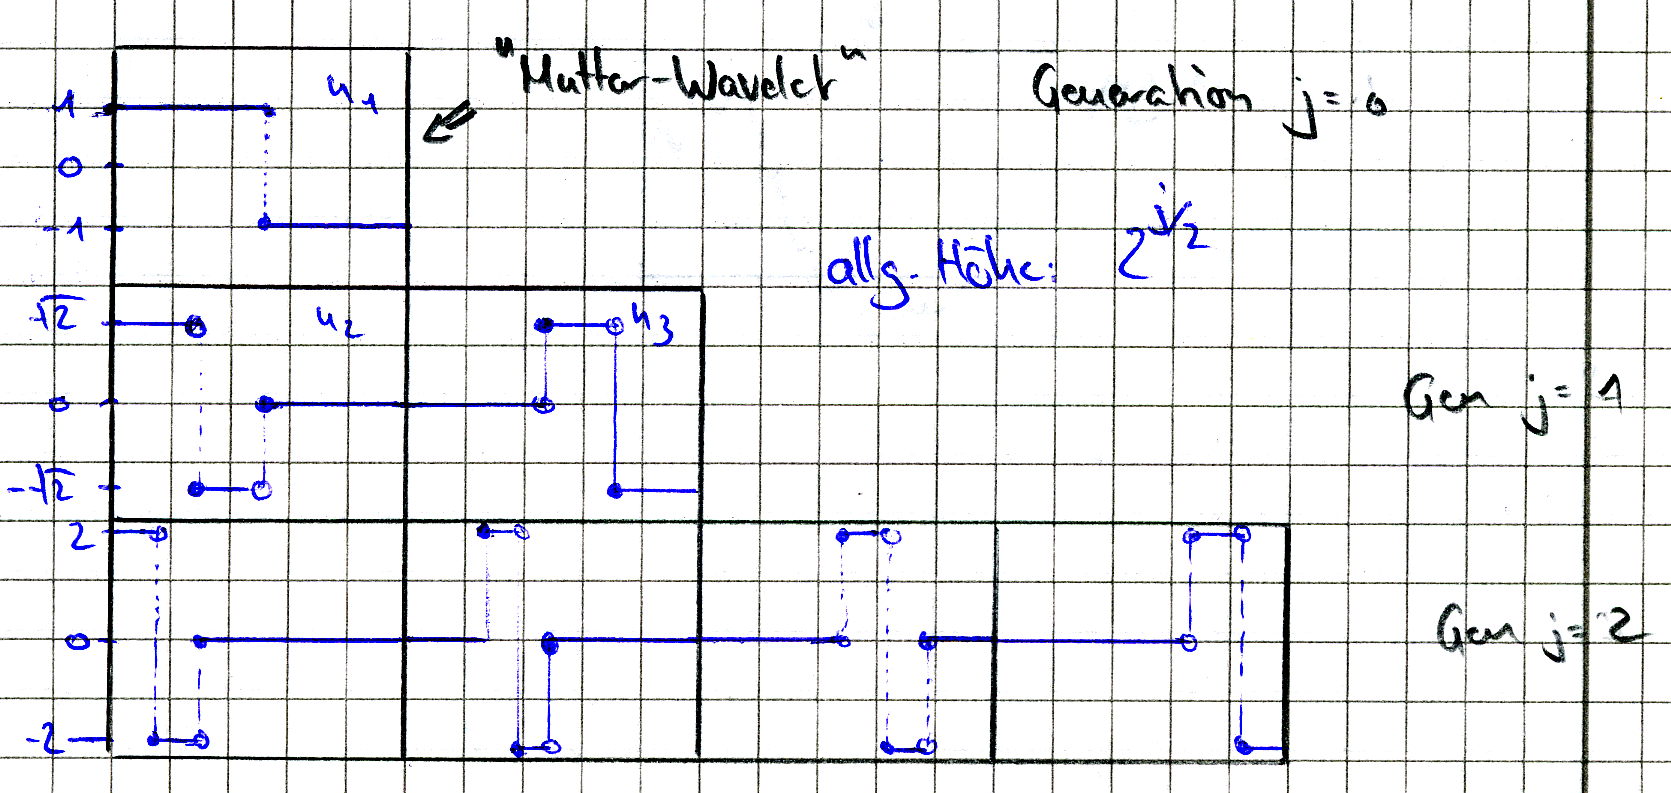
\includegraphics[width=1\textwidth]{./pics/WTHMscan001.png}
\end{document}